\documentclass{../source/Experiment}

\major{信息工程}
\name{姚桂涛}
\title{二极管双平衡混频与吉尔伯特双平衡混频}
\expname{二极管双平衡混频与吉尔伯特双平衡混频}
\stuid{3190105597}
\college{信息与电子工程学院}
\date{\today}
\lab{东4-319}
\course{通信原理实验}
\instructor{金向东、龚淑君}
\grades{}
\exptype{验证性实验}
\partner{叶慷鹏}
\begin{document}
\section{实验目的和要求}
    (1) 掌握二极管双平衡混频器和吉尔伯特双平衡混频器的工作原理
    (2) 测量混频电路各主要参数
    

    \section{实验原理}
    混频是频谱的线性搬移,输出信号与输入信号相比,只是载波频率发生了变化,频谱结构没有变化,输出信号的波形也没有变化。实现混频的基本方法是将两个输入信号相乘。在发射机中使用上混频,本振信号将已调制的中频信号搬移到射频频段。在接收机中使用下混频,通过混频,将接收到的射频信号搬移到中频频段。设混频器的本振输入信号为:
    $$
    v_{L O}(t)=V_{L O} \cos \omega_{L O} t
    $$

    频器的另外一路信号为:
    $$
    v_{i}=V_{i} \cos \omega_{i} t
    $$

    路信号相乘, 得到的输出信号为:
    $$
    v_{o}=\frac{1}{2} V_{L O} V t\left[\cos \left(\omega_{i}+\omega_{L O}\right) t+\cos \left(\omega_{i}-\omega_{L O}\right) t\right]
    $$

    对于发射机系统中的上混频,是把差频滤除,保留和频信号;对于接收机系统中的下混频,是把和频滤除,保留差频信号。

    \subsection{混频器的主要性能指标}
    (1) 混频增益: 混频器的增益定义为混频器输出信号的幅度与输入信号幅度之比,是变频增益。
    (2) 线性度:1dB 增益压缩点:变频增益下降 1dB 时对应的输入信号功率。

    (3) 隔离度: 隔离度一般采用输出信号相对于输入信号的衰减量来表示,以 dB 为单位。

    \subsection{二极管双平衡混频器}
    若二极管两端的电压为 vD(t), 其伏安特性为:
    $$
    i_D = g_DS_1(\omega t)v_D(t)
    $$
    假设在二极管两端所加的电压为$ v_D(t) = v_{LO}(t) + v_i(t)$, $v_{LO}(t) = V_{LO} cos \omega_{LO}t $是本振信号, 为大信号,
    $v_i(t) = V_i cos \omega_it $是小信号。开关函数

    $ S1 (\omega_{LO}t) = \dfrac{2}{\pi} cos \omega_{LO}t −\dfrac{2}{3\pi} cos \omega_{LO}t + \dfrac{25}{\pi}cos \omega_{LO}t − \cdots $

    因此, 作为混频器时, 可以得到本振信号和输入小信号的和频 $\omega_{LO} + \omega i$ 和差频 $\omega_{LO} − \omega i$信号,通过滤波器即可获得所需的混频信号。这种简单的二极管混频电路,输出信号中的组合频率分量比较多,在实际应用中常使用二极管双平衡混频器
    \begin{figure}[H]
        \centering
        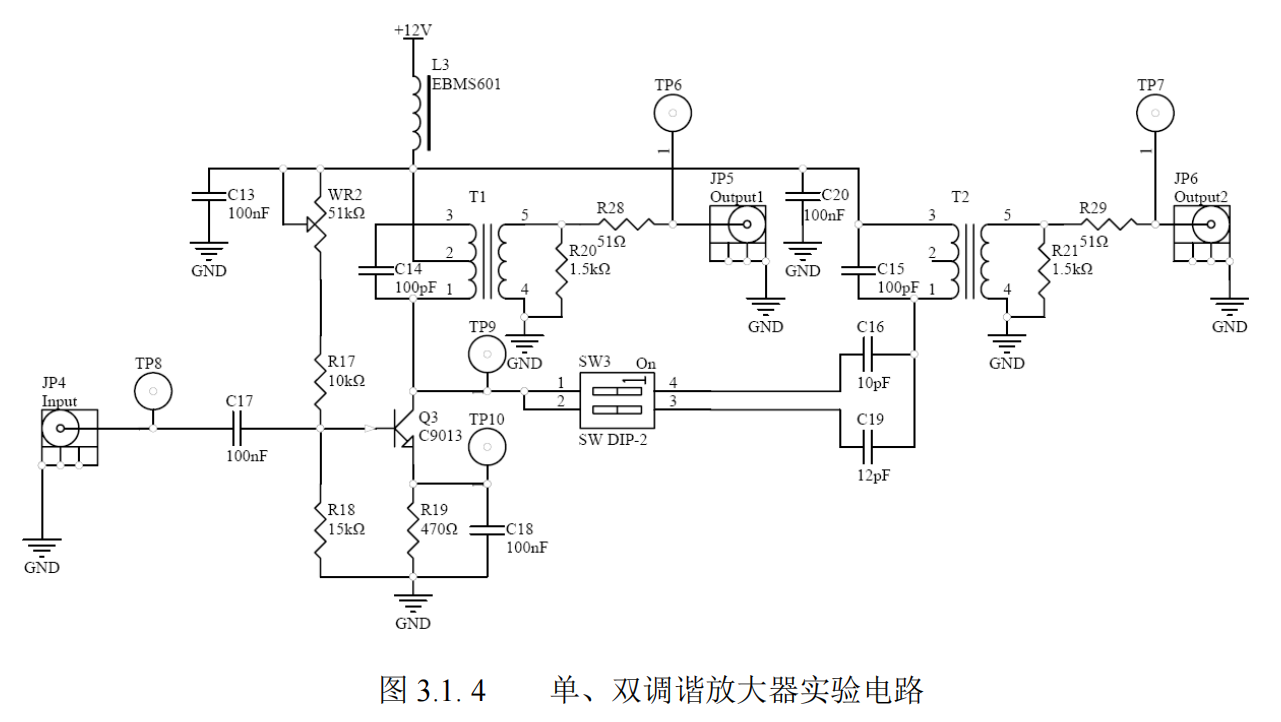
\includegraphics[width = 0.8\textwidth]{pic/fig2.png}
        \caption{二极管双平衡混频电路}
    \end{figure}

    求解回路方程可得整个本振信号周期内流过输出负载上的电流为:

    $$
    i=\left(i_{D 3}-i_{D 4}\right)-\left(i_{D 2}-i_{D 1}\right)=\frac{2 v_{i}(t)}{2 R_{L}+R_{D}} S_{2}\left(\omega_{L O} t\right)
    $$

    式中, $ S_2 (\omega_{LO}t)$ 为频率 $\omega_{LO}$ 的双向开关函数,
    $$
    S_{2}\left(\omega_{L O} t\right)=\frac{4}{\pi} \cos \omega_{L O} t-\frac{4}{3 \pi} \cos 3 \omega_{L O} t+\frac{4}{5 \pi} \cos 5 \omega_{L O} t \cdots
    $$

    因此, 在输出负载电流中存在本振信号与输入小信号的和频 $\omega_{LO} + \omega i$ 和差频 $\omega_{LO} − \omega i$信号。

    \subsection{吉尔伯特双平衡混频器}

    本振信号输入部分是两个差分对管,射频口为一个差分对管。通常,本振口送大信号,Q1、Q2、Q3、Q4组成开关控制电路。射频口送小信号,电路工作在线性放大区。

    \begin{figure}[H]
        \centering
        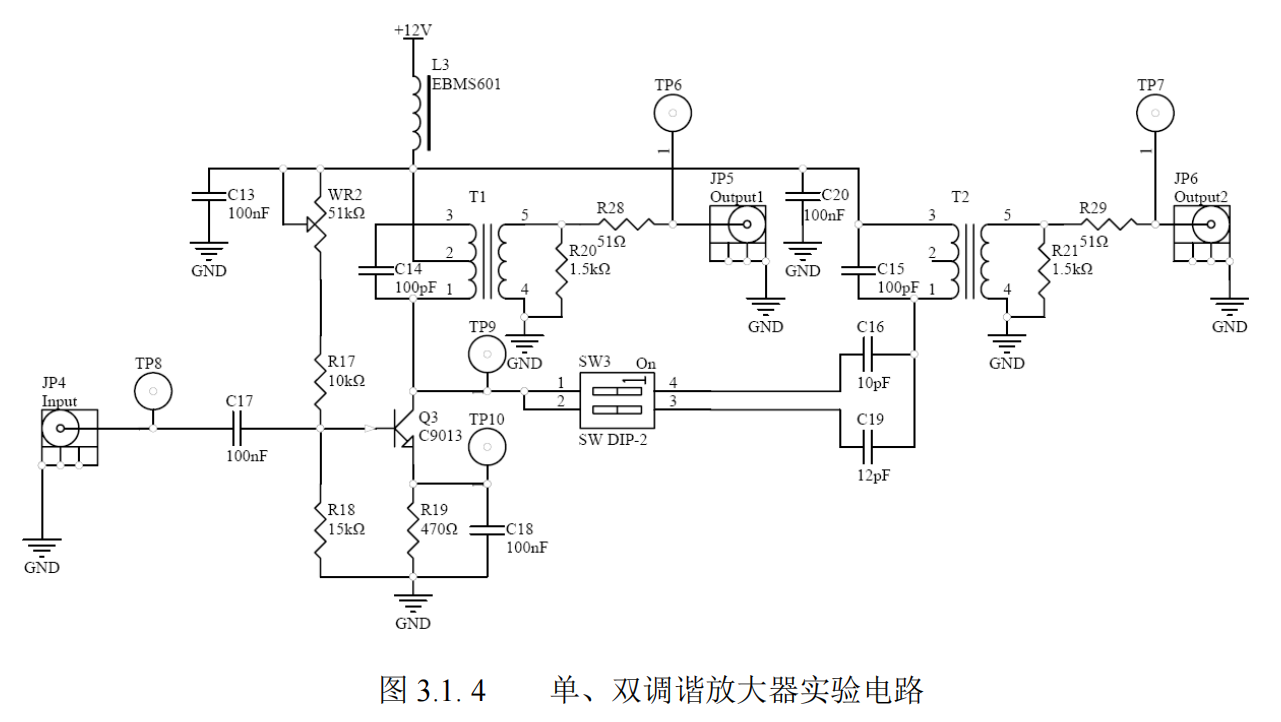
\includegraphics[width = 0.8\textwidth]{pic/fig2.png}
        \caption{吉尔伯特双平衡混频器}
    \end{figure}

    假设流过晶体管 $Q1,Q2,Q3,Q4,Q5,Q6$ 的电流分别是 $i1,i2,i3,i4,i5,i6$, 则中频口的输出电流为:
    $$
    \begin{aligned}
    i &=\left(i_{1}+i_{3}\right)-\left(i_{2}+i_{4}\right)=\left(i_{1}-i_{2}\right)-\left(i_{4}-i_{3}\right) \\
    &=\left(i_{5}-i_{6}\right) \operatorname{th}\left(\frac{q v_{L O}}{2 K T}\right)=I_{0} \text { th }\left(\frac{q v_{L O}}{2 K T}\right) \operatorname{th}\left(\frac{q v_{R F}}{2 K T}\right)
    \end{aligned}
    $$
    对于本振信号为大信号, 射频信号为小信号的情况,
    $$
    t h\left(\frac{q v_{L O}}{2 K T}\right) \approx S_{L O}\left(\omega_{L O} t\right) \quad t h\left(\frac{q v_{R F}}{2 K T}\right) \approx \frac{q v_{R F}}{2 K T}
    $$
    所以,
    $$
    i=I_{0} \frac{q}{2 K T} v_{R F} \cdot S_{L O}\left(\omega_{L O} t\right)
    $$
    将本振信号的开关函数代入上式, 就可以得到本振信号与射频小信号的差频、和频分量, 经过滤波器得变频信号。
    \section{实验电路分析}

    

    二极管双平衡混频器用作上变频混频器,。混频器内部有四个相同的二极管构成环形乘法器,本振信号 LO
    (选用 25MHz)由外部信号源提供,从 JP2 端输入,由传输线变压器转双端输入,中频信号 IF(选用 10.7MHz)
    由外部信号源提供或由 2 号实验板的压控振荡器提供,从 JP4 端输入。混频后的射频信号从 JP3 端输出,经
    过跳线 J4 连接到带通滤波器的输入端 JP5。滤波器选用由 LC 实现的带通滤波器,其中心频率为 36MHz,带
    宽约 8MHz。其作用是将上变频输出信号中的和频信号(35.7MHz)滤出,从 JP6 输出。
    \begin{figure}[H]
        \centering
        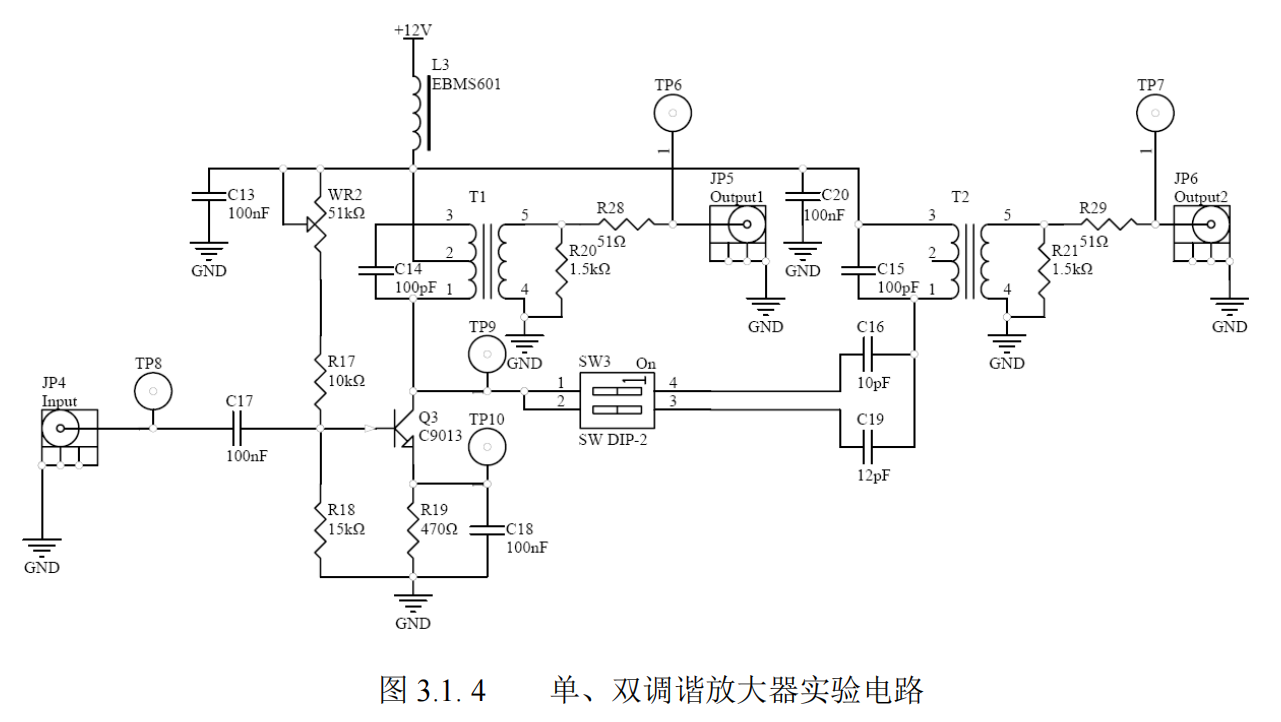
\includegraphics[width = 0.8\textwidth]{pic/fig2.png}
        \caption{二极管双平衡混频实验电路}
    \end{figure}

    下变频电路为吉尔伯特双平衡混频结构,实验电路采用 MC1496 双平衡调制解调芯片,如图 3.5. 5 所示,MC1496 芯片的内部由吉尔伯特单元电路构成。下变频电路的射频信号(35.7MHz)由外部信号源提供,或通过跳线 J5 连接带通滤波器,从上变频电路的输出中得到。25MHz 的本振信号由外部信号源提供,从 JP2 端输入,混频输出信号经过 10.7MHZ 的陶瓷滤波器滤波,在 JP8 端得到中频输出信号。

    \begin{figure}[H]
        \centering
        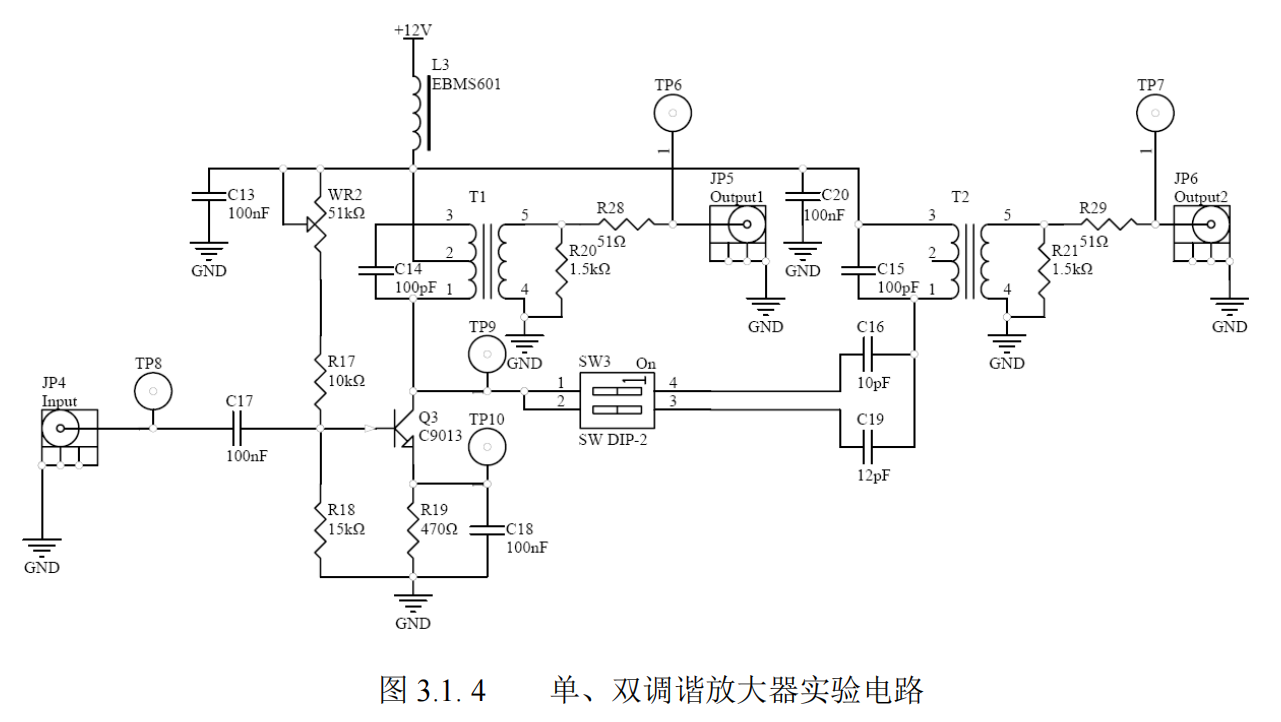
\includegraphics[width = 0.8\textwidth]{pic/fig2.png}
        \caption{二极管双平衡混频实验电路}
    \end{figure}

    \section{实验设备}
        \begin{enumerate}
            \item 实验办No01 \, 1块
            \item 信号源1台
            \item 双踪示波器1台
            \item 频谱分析仪(含TG)1台
            \item 万用表1台
        \end{enumerate}
        
    \section{实验数据与结果分析}
        \subsection{二极管双平衡混频器上变频实验}
            \subsubsection{混频器变频增益测量}
            
            JP4 端输入幅度为 0dBm,频率为 10.7MHz 的正弦信号作为中频输入信号。设定频谱分析仪中心频率为35.7MHz,设定扫频带宽 SPAN 为 50kHz,分辨率带宽 RBW 为 1kHz,读取输出信号中和频分量的幅度(功率),计算混频增益。
            
            \begin{figure}[H]
                \centering
                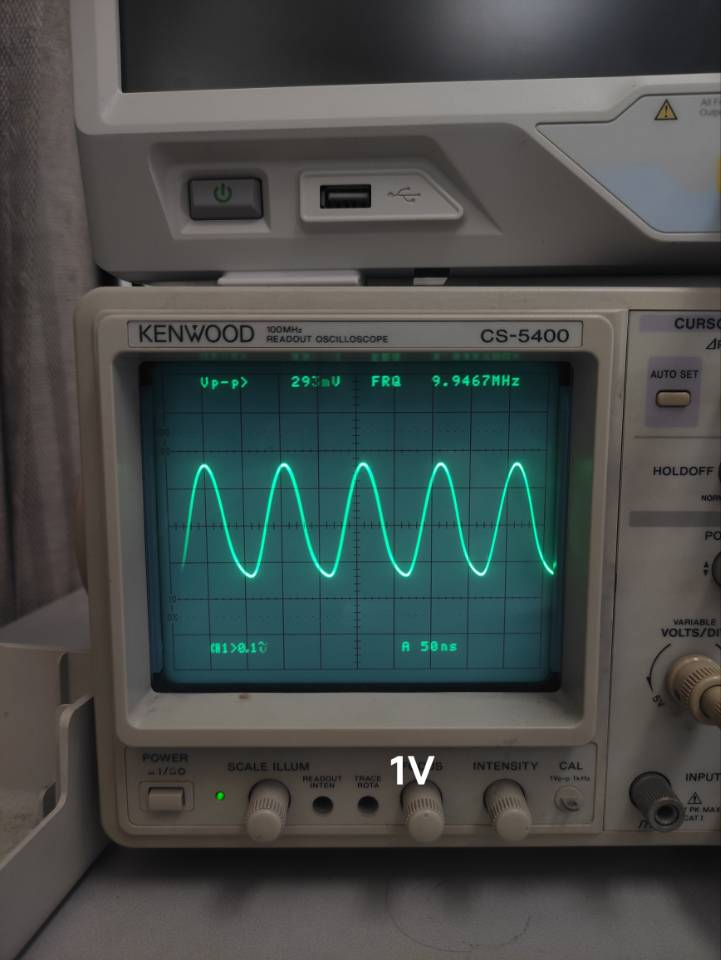
\includegraphics[width = 0.6\textwidth]{4}
                \caption{ 0dBm 输入时的输出信号}
            \end{figure}
            从图中可以读出,和频分量的幅度为-7.16dBm,因此混频增益为-7.16dB。后来我们改变了本振信号的幅
            度,分别测试了本振信号幅度为 0dBm 和-10dBm。测量结果如下图:
            \begin{figure}[H]
                \centering
                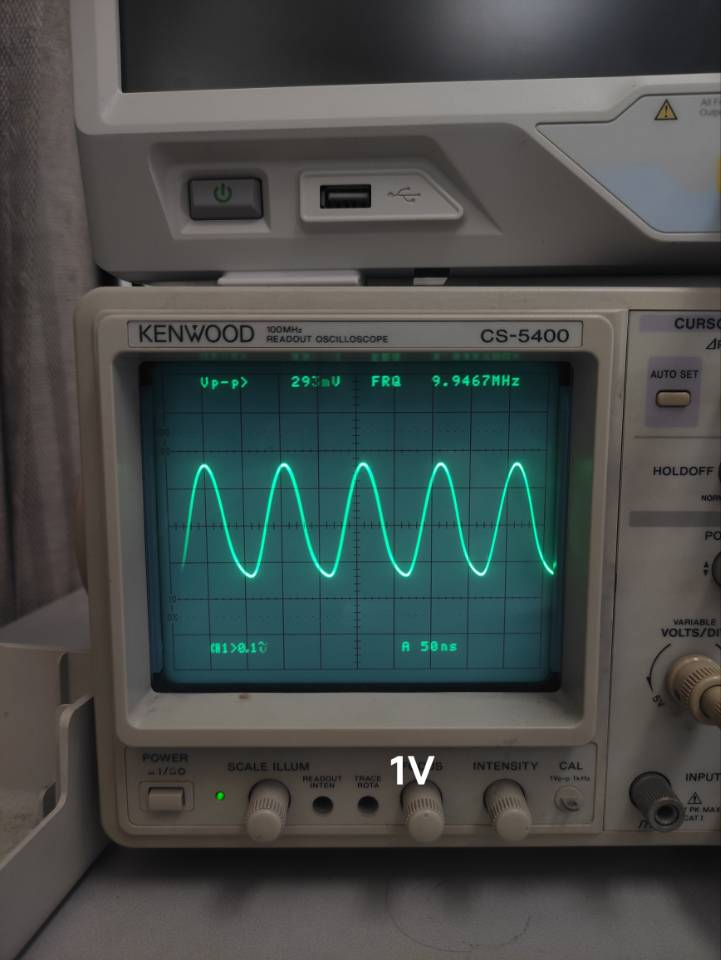
\includegraphics[width = 0.6\textwidth]{4}
                \caption{0dBm 输入时的输出信号}
            \end{figure}

            本振幅度为 0dBm 时,混频增益为-11.16dB。

            \begin{figure}[H]
                \centering
                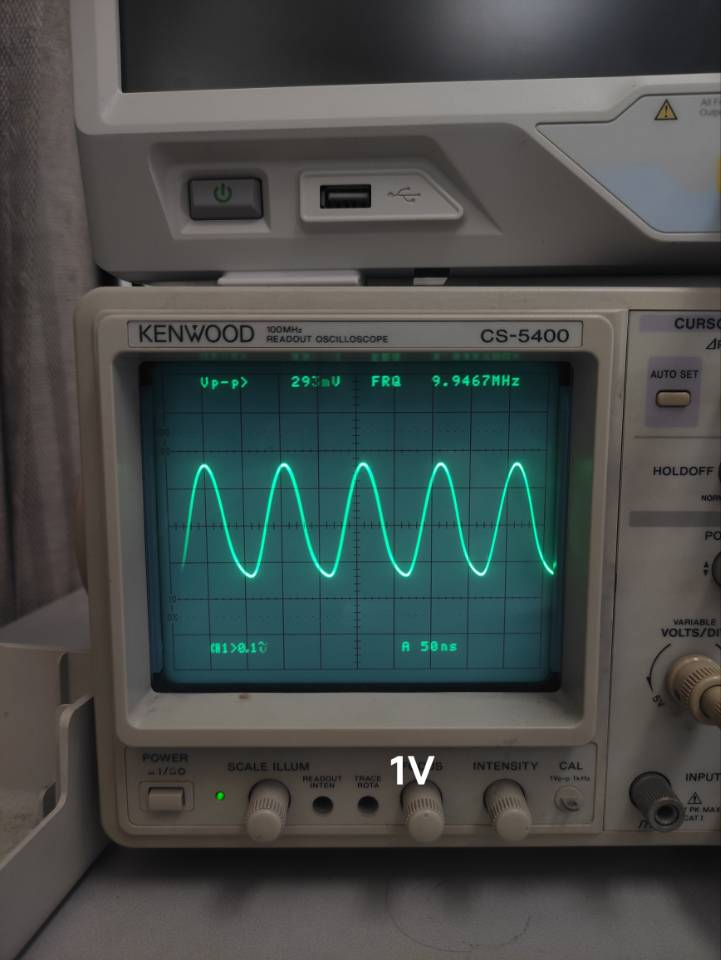
\includegraphics[width = 0.6\textwidth]{4}
                \caption{-10dBm 输入时的输出信号}
            \end{figure}

            本振幅度为-10dBm 时,混频增益为-21dB。因此混频增益随本振信号幅度增加而增加。本振信号幅度越高,混频增益越大。

            输入的中频信号也可采用 AM 调制信号或 FM 调制信号。若是 AM 调制信号,可设置调制信号频率为5kHz,调制度为 50\%;若是 FM 调制信号,可设调制信号为 1kHz,调制频偏为 4.5kHz。在混频输出端分别观测以上 AM 调制与 FM 调制的信号频谱,并计算混频增益。

            \begin{figure}[H]
                \centering
                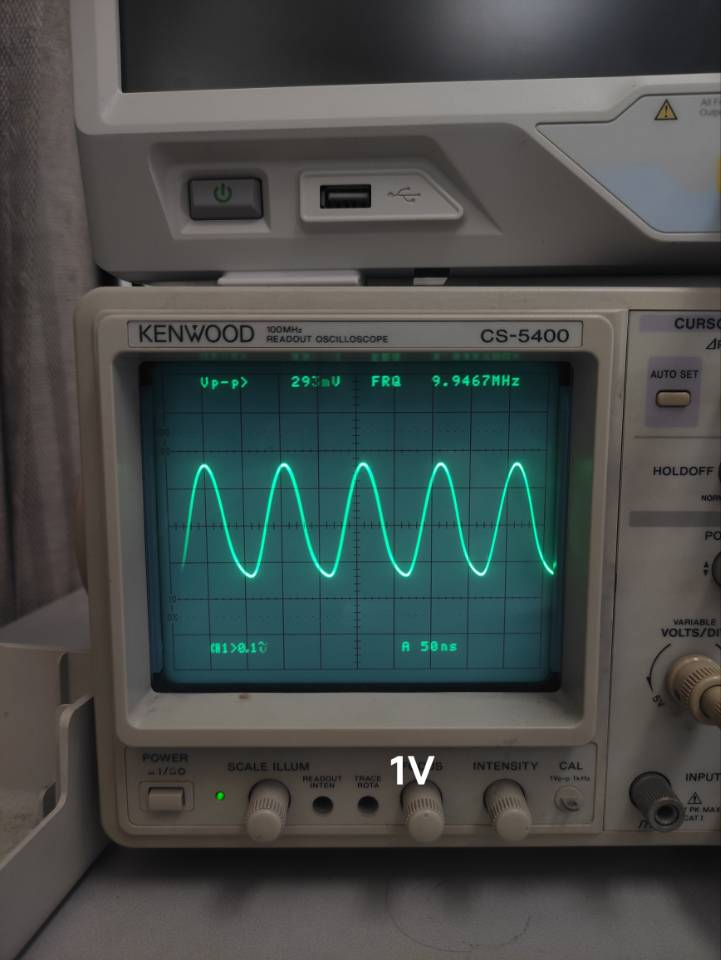
\includegraphics[width = 0.6\textwidth]{4}
                \caption{输入 AM 调制信号时输出波形}
            \end{figure}

            混频增益为-11.54dB。

            \begin{figure}[H]
                \centering
                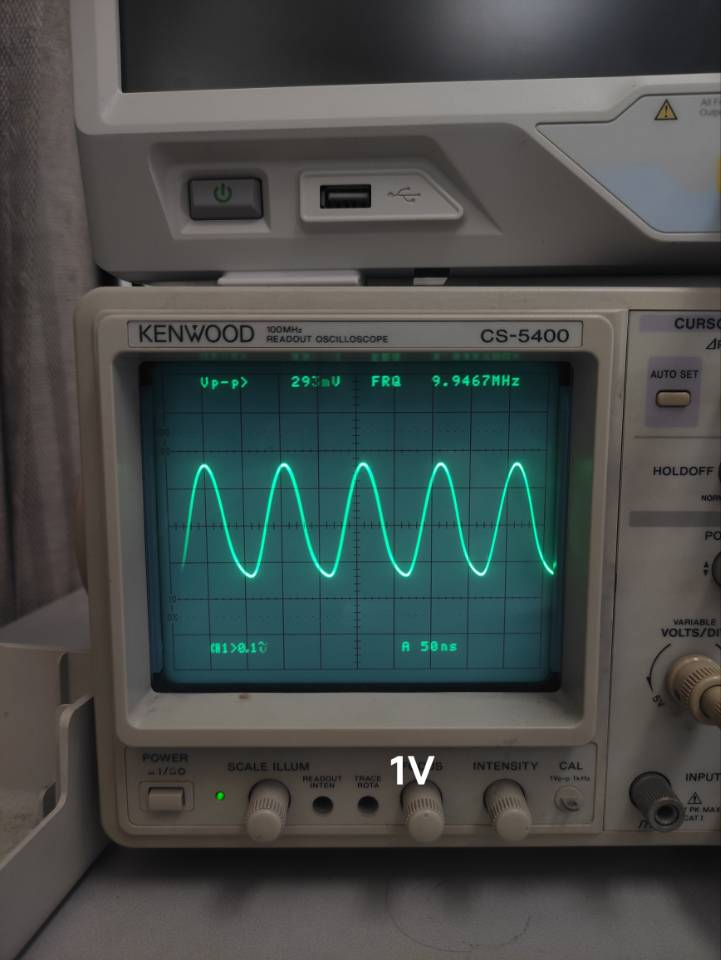
\includegraphics[width = 0.6\textwidth]{4}
                \caption{输入 FM 调制信号时输出波形}
            \end{figure}
            混频增益为-13.76dB。
        \subsubsection{隔离性能测试}
        在使用频谱仪测量混频增益的基础上,在混频输出端 JP3,观察在本振频率点 25MHz,中频 10.7MHz 的信号分量大小,分别计算混频输出端对本振信号和中频信号的隔离度。

        25MHZ 的输出分量为:-48.46dBm

        隔离度为-48.46dBm-10dBm=-58.46dB

        10.7MHz 的输出分量为-23.77dBm

        隔离度为-23.77dBm-0=-23.77dB
        
        \subsubsection{带通滤波性能测试}

        保持以上输入信号不变,连接跳线 J4,滤波器设成 LC 带通滤波器(将 J1 和 J2 的第 6 位跳线接通,J3的 1-2 脚连通);将频谱分析仪的中心频率设为 25MHz,扫宽设为 40MHz;频谱仪输入分别连接 JP3 和 JP6,观测混频信号通过滤波器滤波前后的频谱,测量滤波前后和频与差频的信号幅度。

        \begin{figure}[H]
            \centering
            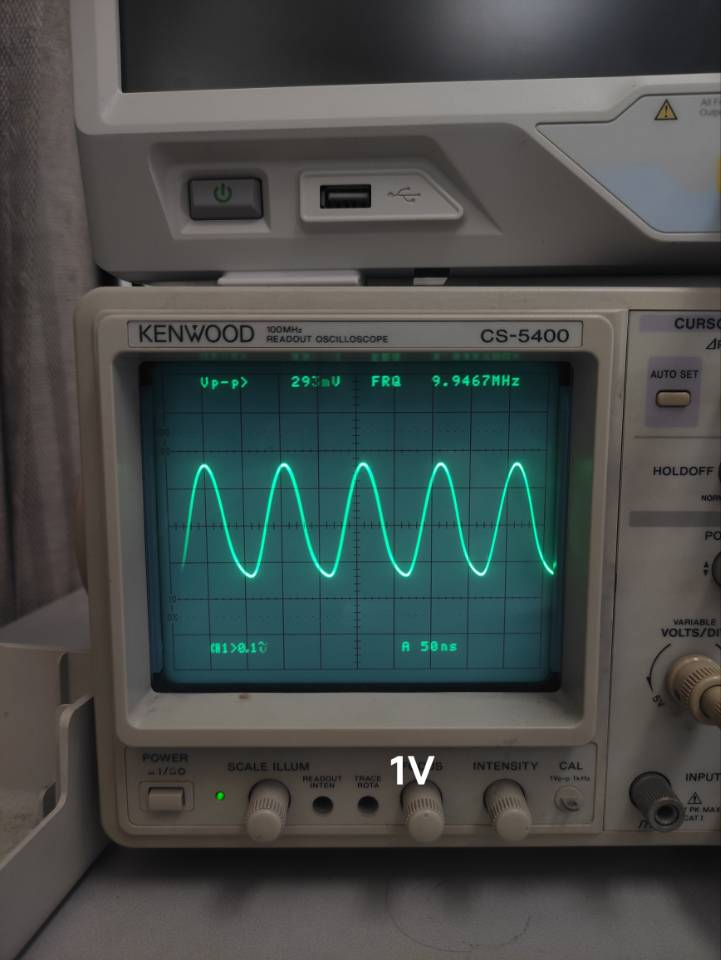
\includegraphics[width = 0.6\textwidth]{4}
            \caption{滤波前和频}
        \end{figure}

        \begin{figure}[H]
            \centering
            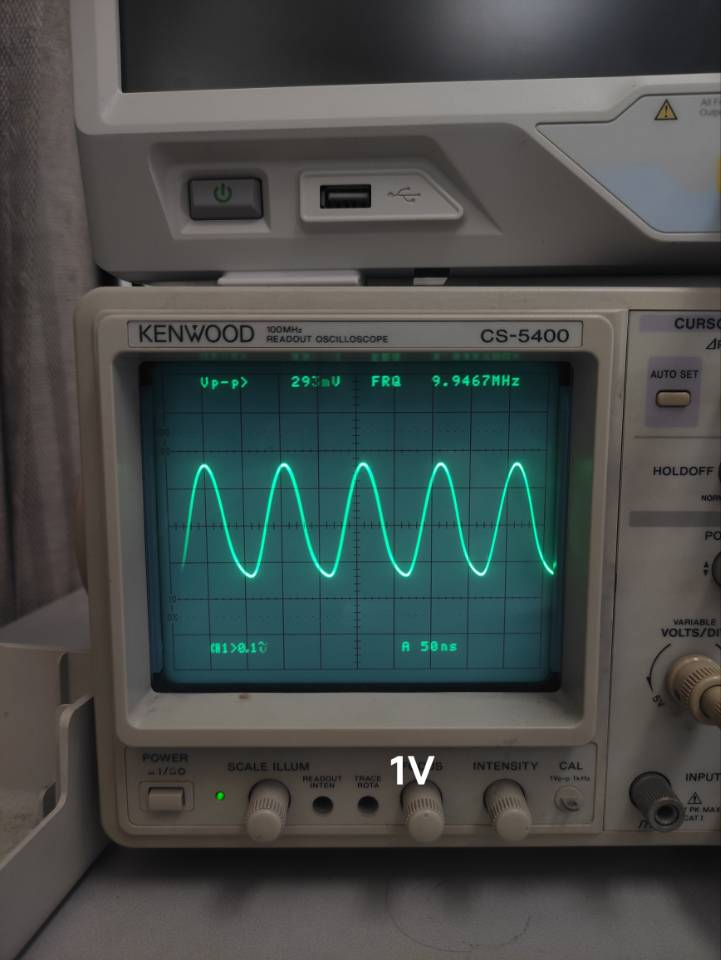
\includegraphics[width = 0.6\textwidth]{4}
            \caption{滤波前差频}
        \end{figure}

        \begin{figure}[H]
            \centering
            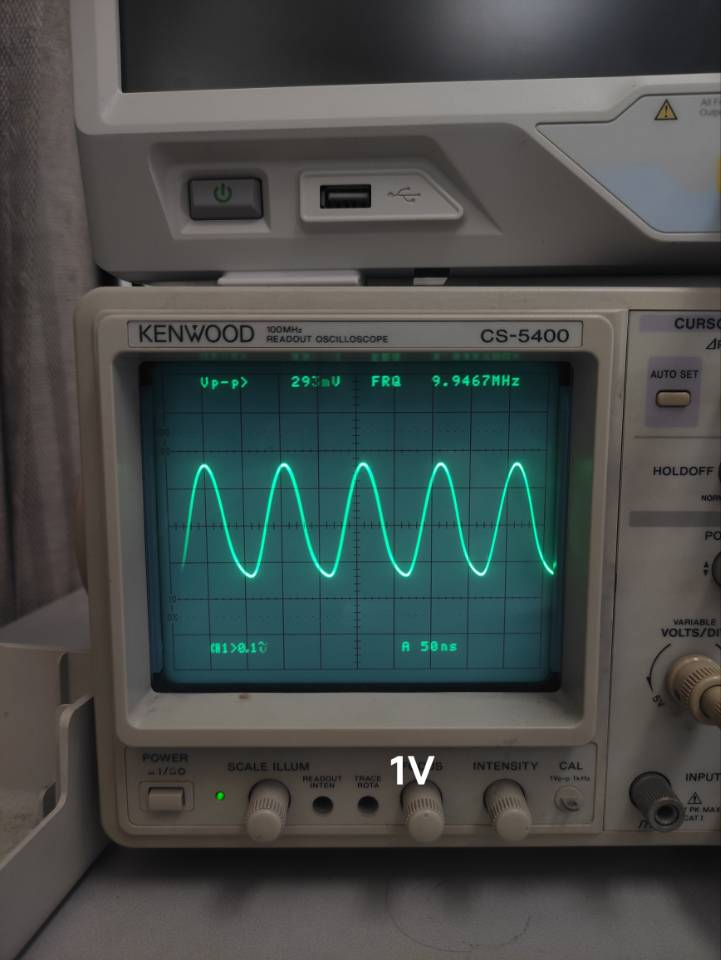
\includegraphics[width = 0.6\textwidth]{4}
            \caption{滤波后和频}
        \end{figure}

        从图中可以看出滤波前和频信号幅度为-10.08dBm,滤波前差频信号为-6.58dBm。滤波后和频信号幅度为21.56dBm,差频信号幅度为 0。和频信号被滤除。

    \subsection{吉尔伯特双平衡混频器下变频实验}
        \subsubsection{混频器变频增益测量}
        设定本振信号的幅度为 10dBm;设定射频信号的幅度为-10dBm;设定频谱分析仪中心频率为 10.7MHz,扫描带宽 SPAN 为 50KHz,在 JP8 端用频谱分析仪测量混频器的中频输出,计算混频增益。

        \begin{figure}[H]
            \centering
            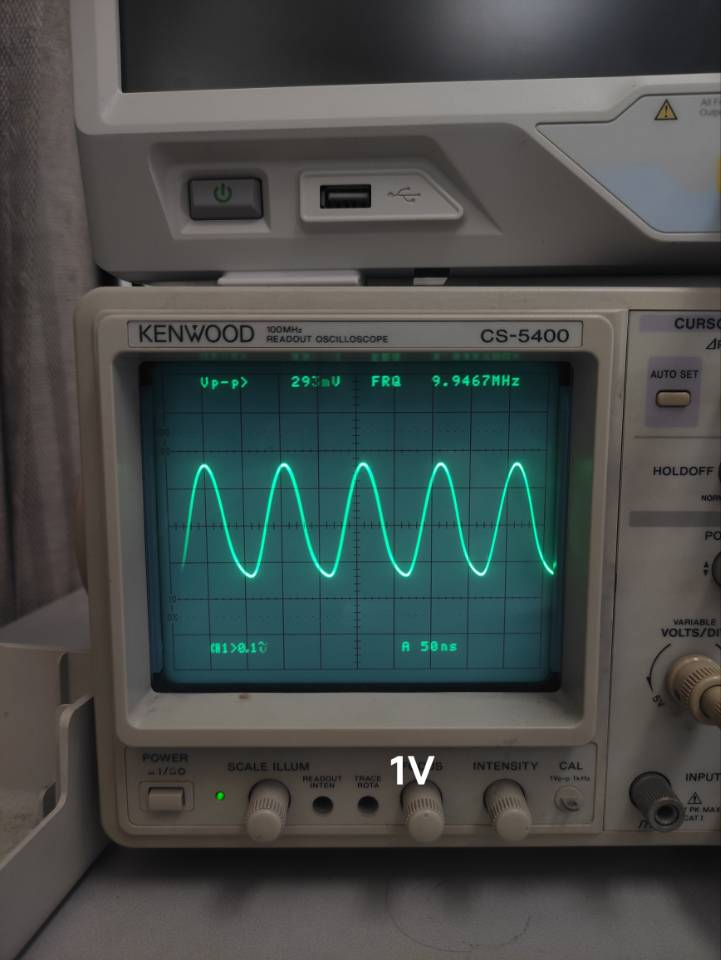
\includegraphics[width = 0.6\textwidth]{4}
            \caption{吉尔伯特双平衡混频器混频增益}
        \end{figure}

        可以看到输出信号为-18.09dBm,因此混频增益为-8.09dBm。

        \subsubsection{混频器 1dB 压缩点测量}
        
        在本振信号幅度为 10dBm 的条件下,采用信号源作为射频输入,改变输入信号的幅度,测量输出信号的幅度,填入下表,计算 1dB 压缩点。

        \begin{table}[H]
            \begin{tabular}{|c|c|c|c|c|c|c|c|c|c|c|}
            \hline
            输入功率(dBm) & -25    & -24    & -23    & -22   & -21    & -20    & -19    & -18    & -17    & -16    \\ \hline
            输出功率(dBm) & -29.17 & -28.36 & -27.45 & -26.5 & -25.61 & -24.67 & -23.85 & -22.98 & -22.15 & -21.38 \\ \hline
            增益(dB)    & -4.17  & -4.36  & -4.45  & -4.5  & -4.61  & -4.67  & -4.85  & -4.98  & -5.15  & -5.38  \\ \hline
            输入功率(dBm) & -15    & -14    & -13    & -12   & -11    & -10    & -9     & -8     & -7     & -6     \\ \hline
            输出功率(dBm) & -20.66 & -20.03 & -19.45 & -18.9 & -18.47 & -18.06 & -17.75 & -17.54 & -17.33 & -17.18 \\ \hline
            增益(dB)    & -5.66  & -6.03  & -6.45  & -6.9  & -7.47  & -8.06  & -8.75  & -9.54  & -10.33 & -11.18 \\ \hline
            \end{tabular}
        \end{table}

        从上表中可以看出,刚开始随着输入功率的增大,增益基本上为恒定值在-4dB 左右,然后到输入功率增大到-17dBm 的时候,输出功率为-22.15dBm,此时增益为-5.15dB,此点即为 1dB 压缩点。
    \section{思考题}
	    \subsection{混频器的主要性能指标有哪些?}
        
        \subsection{吉尔伯特双平衡混频器与二极管双平衡混频器相比,优势有哪些?}

        \subsection{混频器变频增益主要受哪些因素的影响?}
	
\end{document}